\documentclass[a4paper,8pt]{article}
\usepackage[utf8]{inputenc}
\usepackage[english]{babel} %language
\usepackage[
backend=bibtex
]{biblatex}
\addbibresource{references.bib}
\usepackage{amssymb}
\usepackage{listings}
\usepackage{xcolor}
\usepackage{array}
\usepackage{float}
\usepackage{amsmath}

%CodeColours
\definecolor{codegreen}{rgb}{0,0.6,0}
\definecolor{codegray}{rgb}{0.5,0.5,0.5}
\definecolor{codepurple}{rgb}{0.58,0,0.82}
\definecolor{backcolour}{rgb}{0.95,0.95,0.92}
\definecolor{codeblue}{rgb}{0,0,0.80}



%Codestyle
\lstdefinestyle{mystyle}{
	backgroundcolor=\color{backcolour},   
	commentstyle=\color{codegreen},
	keywordstyle=\color{orange},
	numberstyle=\tiny\color{codegray},
	stringstyle=\color{codepurple},
	basicstyle=\ttfamily\footnotesize,
	identifierstyle=\color{codeblue},
	breakatwhitespace=false,         
	breaklines=true,                 
	captionpos=b,                    
	keepspaces=true,                 
	numbers=left,                    
	numbersep=5pt,                  
	showspaces=false,                
	showstringspaces=false,
	showtabs=false,                  
	tabsize=2,
	basicstyle=\scriptsize
}
%Set style
\lstset{style=mystyle}

%Images and similar
\usepackage{graphicx}
\graphicspath{.}

%timeline
\usepackage{tikz}
\usetikzlibrary{snakes}
\usepackage{rotating}

\title{Root-Causing and Event Identification Through Sensor Data}
\author{Simon dos Reis Spedsbjerg : sispe20@student.sdu.dk\\ {\small Advisor: Aslak Johansen : asjo@mmmi.sdu.dk}}

\newcommand{\Phases}{8 }
\newcommand{\phaseq}{Related Work}
\newcommand{\phasew}{Data Collection}
\newcommand{\phasee}{Analysis}
\newcommand{\phaser}{Design}
\newcommand{\phaset}{Implementation}
\newcommand{\phaseSetup}{Setup}
\newcommand{\phasey}{Evaluation}
\newcommand{\phaseu}{Conclusion}

\usepackage{biblatex}


\usepackage[acronym]{glossaries}
\newacronym{reps}{REPS}{Relational Event Prediction System}
\newacronym{gui}{GUI}{Graphical User Interface}

\begin{document}
	\maketitle
	\section{Context}
		
			In this project, some definitions has to be agreed upon to achieve best understanding of the project.
			\begin{itemize}
				\item \textbf{Change of State}, a change of state is one or more of an objects attributes has changed. A change of state might be a concern which one would want to act on, i.e. planning reasons, mitigation or avoidance.
				\item \textbf{Event}, an event is the change of the state of an object, it has one or more inputs and outputs. The input of an event can vary, have levels (e.g. low, medium and high), have a value above or below a threshold, consider time and state, or be boolean. An event output is a function over the events inputs.
				\item \textbf{Ongoing Event}, an event is considered ongoing if the change has not reversed to a normal state, normal state being the state the object was before the event.
				\item \textbf{Value}, A value is produced by a sensor or an event.
				\item \textbf{Event Rule}, Event rules are logic statements that are expected to have be fulfilled before an event can occur, an event rule can be attached to one or more events. An event can occur without the rules being fulfilled, but this means the expectations are wrong. The Event might not occur while the event rules are fulfilled, which means the expectations are wrong.%And the system needs to be revised
				\item \textbf{Trigger} An event is triggered when the change of state occurs. When an event is triggered, it emits a boolean value. (Figure \ref{fig:eventInAOut})
			\end{itemize}
		I define \gls{reps} as a system that attempts to predict an event based on changes to one or more values which the value shares any form of relation with. 
		\begin{figure}[!h]
			\centering
			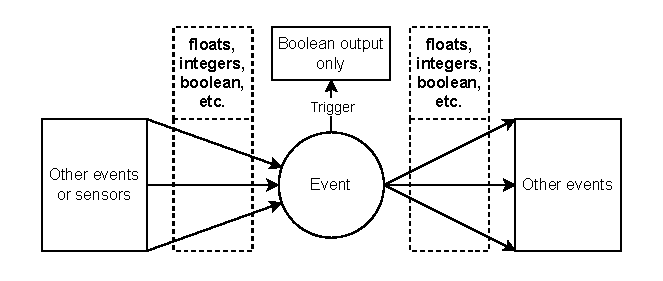
\includegraphics[width=.8\textwidth]{EventTrigger}
			\caption{Event Input and Outputs}
			\label{fig:eventInAOut}
		\end{figure}
		\newpage
		Using \gls{reps} we can predict events based on the event rules of each event. Given an ongoing event, \gls{reps} is able to backtrace and determine the causes of the ongoing event.
		
		A sensor does not have any input nodes(Figure \ref{fig:prediction}), it is the first producer of data which feeds the rest of the event network.
		\begin{figure}[!h]
			\centering
			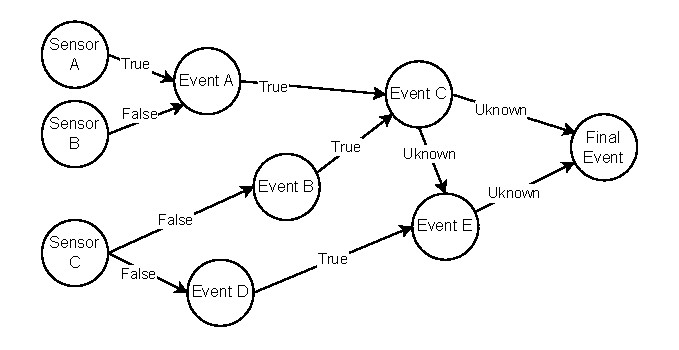
\includegraphics[width=.9\textwidth]{Events}
			\caption{Predicting events based on current events and the event rules. Unknown relations is relations which has not been evaluated yet.}
			\label{fig:prediction}
		\end{figure}
		
		The amount of data collected is ever-increasing, and analysis and predictive systems ever becoming more dependent on the quality of their input data. Faulty (caused by an error in the system) or abnormal (caused by an event that does not represent normal operations in the system by having high or low values) data may invalidate the analysis that is performed on the data. An abnormal data point may indicate that another part of the system is the cause.
		An expected event that never occurs (i.e. according to event rules, the event should be triggered but is not) in one place, could mean an event in another place has been triggered. We could expect that a decrease in outside temperature to lead to an increase in power consumption for heating and thus a higher heating bill. If an increase in power consumption is not observed, then this may indicate that the occupants are dressing warmer or are using another heat source that we are not measuring. An event not being triggered even though its rules are fulfilled can indicate:
		\begin{itemize}
			\item A sensor is not producing correct data.
			\item The \gls{reps} logic is wrong and needs readjustment.
		\end{itemize}
		
		Sensors that give data that is abnormal might indicate the need for maintenance\cite{MUKHERJEE2024102444}, an upcoming domain specific event, or a successful intrusion into some parts of the system\cite{MR2022103046}. Information to predict events or needs has become an interest in many sectors. Mukherjee, A\cite{MUKHERJEE2024102444} cites the transport, manufacturing, water, and power domains, while they try to predict maintenance for container cranes. Predicting ongoing events might be important when it comes to cyberattacks. Gauthama et al. worked on predicting an ongoing event of a possible attack in a water treatment plant using its multipoint IoT sensory system\cite{MR2022103046}.
		
		\gls{reps} thereby attempts to predict future and ongoing events based on the event rules and the current readings from the sensors. \gls{reps} is also able to backtrace once an event is triggered to determine the cause of the event. It will predict future events by measuring the sensors' values and by the event rules. It will try to determine the root cause of an event by removing events from the set of possible events by querying by their event rules (Figure \ref{fig:EventRuleBroken}).
		\begin{figure}[!h]
			\centering
			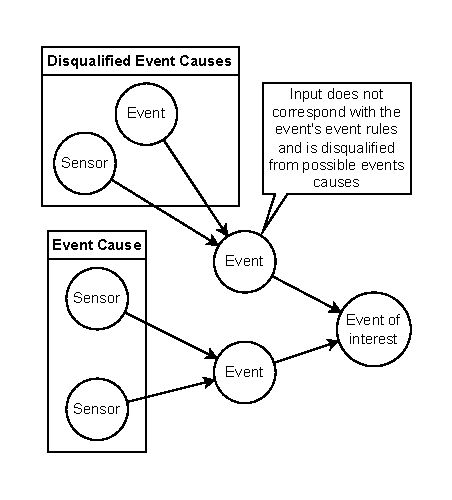
\includegraphics[width=.7\textwidth]{EventRuleBroken}
			\caption{Cause determination of ongoing event}
			\label{fig:EventRuleBroken}
		\end{figure}
		\newpage
	\section{Problem}
		Research Questions:
		\begin{itemize}
			\item RQ0: How should a \gls{reps} be constructed?
			\item RQ1: How well does \gls{reps} perform in a system with multiple sensors?
			\item RQ2: What advantages and disadvantages does \gls{reps} have compared to other solutions?
		\end{itemize}
	\section{Approach}
		To find answers to the research questions, I can choose either of 2 approaches depending on availability of data: 
		\begin{itemize}
			\item \textbf{Data Based Prediction}, using the data I will simulate a real-life system using separate computers as individual systems where the \gls{reps} will try to make predictions.
			\item \textbf{Digital Twin}, defined as digital model of a real world physical system. The second approach is to set up digital twins of systems that would generate data live. This will require constant attention that the digital twins does not give an unfair advantage to \gls{reps} to avoid bias.
		\end{itemize}
		Either case, the approach chosen will be compared to other available algorithms which solves same or similar problem.
		Then a comparison between the \gls{reps} and other available algorithms is performed where they will be measured for any relevant attributes in performing their task in predicting future events and thereby answering the research questions.
		
		The \textbf{Digital Twin} approach is preferred because it would grant me the ability to create a more varied but realistic scenarios that would be rare to occur in the real world. The \textbf{Data Based Prediction} is more accurate to the real world as this was what real sensors would be giving as a result.
	\section{Timeline}
	I intend to go into \Phases phases during this project. This timeline will most likely change during the project as many unknowns still exists, but it serves as a subjective view of the time needed for the different phases based on my previous experience.
		\begin{enumerate}
			\item \textbf{\phaseq}, develop a clear and thorough understanding of the current state of research in anomaly detection and 'fault detection and diagnosis' by creating a systematic literature review of the subjects.
			\item \textbf{\phasew}, Collect or create relevant data depending on the results of the \phaseq \space which is relevant to the subject. As the results will be drawn on the solution's ability to handle the data, the quality of the data has a high impact on the project.
			\item \textbf{\phasee}, analyse the problem with the help of software engineering methods based on the \phaseq \space results.
			\item \textbf{\phaser}, design a solution to the problem specified in the \phasee \space phase with software engineering methods so it can be efficiently implemented.
			\item \textbf{\phaset}, develop the project based on the results of the \phasee \space and the \phaser \space using software engineering methods. This includes setup for any experimentations.
			\item \textbf{\phaseSetup}, the setup may involve many tools which need setup, this could be for stress testing, having several data producers on each their own services. The setup's purpose is to have all small prerequisites ready for the \phasey \space phase.
			\item \textbf{\phasey}, how well does the solution fulfil the requirements determined in the \phasee \space phase and does it implement all features which is deemed critical.
			\item \textbf{\phaseu}, Answer the research questions and draw a conclusion.
		\end{enumerate}
	
	In the following, we see the expected timeline for the project.\newline
	%Timeline
	\begin{center}
			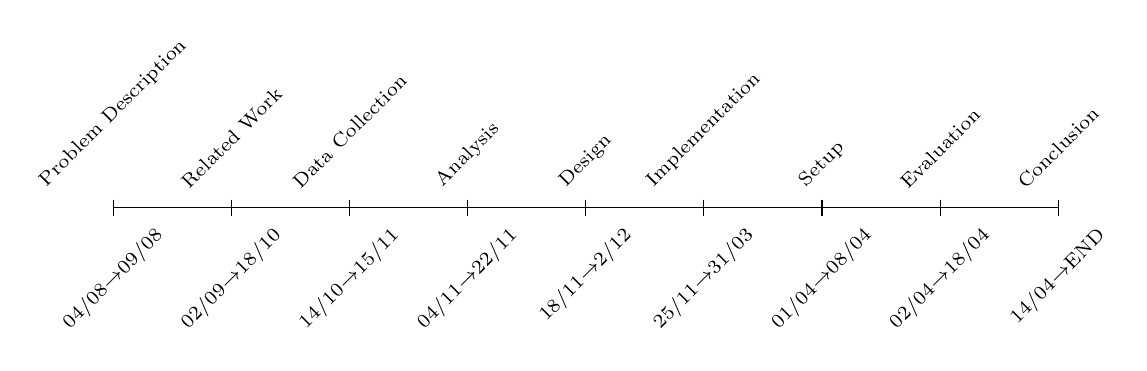
\begin{tikzpicture}
			%create the line
			\draw (-6,0) -- (6,0);
			
			%vertical lines
			\foreach \x in {-6, -4.5, -3, -1.5, 0, 1.5, 3, 4.5, 6}
			\draw (\x cm, 3pt) -- (\x cm, -3pt); %Size of the points in the timeline
			
			%draw
			\draw (-6,0) node[below=3pt] {\begin{turn}{45}\scriptsize 04/08$\rightarrow$09/08\end{turn}}
			node[above=3pt] {\scriptsize\begin{turn}{45}Problem Description\end{turn}}; %start date
			\draw (-4.5,0)
			node[below=3pt] {\begin{turn}{45}\scriptsize 02/09$\rightarrow$18/10\end{turn}}
			node[above=3pt] {\scriptsize\begin{turn}{45}\phaseq\end{turn}};
			
			\draw (-3,0)
			node[below=3pt] {\begin{turn}{45}\scriptsize 14/10$\rightarrow$15/11\end{turn}}
			node[above=3pt] {\scriptsize\begin{turn}{45}
					\phasew
			\end{turn}};
			
			\draw (-1.5,0)
			node[below=3pt] {\begin{turn}{45}\scriptsize 04/11$\rightarrow$22/11\end{turn}}
			node[above=3pt] {\scriptsize\begin{turn}{45}
					\phasee
			\end{turn}};
			
			\draw (0,0)
			node[below=3pt] {\begin{turn}{45}\scriptsize 18/11$\rightarrow$2/12\end{turn}}
			node[above=3pt] {\scriptsize\begin{turn}{45}
					\phaser
			\end{turn}};
			
			\draw (1.5,0)
			node[below=3pt] {\begin{turn}{45}\scriptsize 25/11$\rightarrow$31/03\end{turn}}
			node[above=3pt] {\scriptsize\begin{turn}{45}
					\phaset
			\end{turn}};
			
			\draw (3,0)
			node[below=3pt] {\begin{turn}{45}\scriptsize 01/04$\rightarrow$08/04\end{turn}}
			node[above=3pt] {\scriptsize\begin{turn}{45}
					\phaseSetup
			\end{turn}};
			
			\draw (4.5,0)
			node[below=3pt] {\begin{turn}{45}\scriptsize 02/04$\rightarrow$18/04\end{turn}}
			node[above=3pt] {\scriptsize\begin{turn}{45}
					\phasey
			\end{turn}};
			
			\draw (6,0) node[below=3pt]{\begin{turn}{45}\scriptsize 14/04$\rightarrow$END\end{turn}} node[above=3pt] {\scriptsize\begin{turn}{45} \phaseu \end{turn}};%end date
		\end{tikzpicture}
	\end{center}
	Every 1-4 weeks a plan will be made detailing the coming weeks' task. Each time a plan is made, the previous weeks will be documented on what went well, okay, not so well, and terribly. This is so the supervisor and I can create a perspective and course correct if need be.
	
	The plan is to hold meetings with the supervisor every week, an agenda will be send to the supervisor at minimum 48 hours before the meeting.

	
	\section{Preliminaries/Feasibility}
		The project will have a high chance of success based on the risk analysis and as long the mitigation tactics are used.
	
		\subsection{Risk analysis}
			The risk levels are as follows, insignificant, very low, low, medium, high, very high. This is the likelihood of the risk coming true. An impact value is also set and it has the same levels as the risk levels. Mitigation is the tactic and how well it can be mitigated if the risk were to happen. All these factors will be taken into consideration throughout the project's lifetime based on the cost-benefit.
			{\scriptsize
			\begin{center}
				\begin{tabular}[!h]{|m{8em}|m{6em}|m{5em}|m{5em}|m{5em}|m{9em}|}
					\hline
					Risk Type & Description & Risk & Impact & Mitigation & Comments \\ \hline
					Missing Related work & There is not enough related work to form a proper ground for research & Insignificant & Very high & Reformulate research question & Already from the research that I have read for this topic, it is clear that there is more than enough. \\ \hline
					Unable to gather data for simulations & Either I am able to find the data or I will have to set up some form of a digital twin. & Medium & Medium & Set up digital twins; what the twin is of will be decided after going through related work & The twin is not intended to fit perfectly with the system that I intend to implement, it is supposed to be used to decide whether it is in general a possible solution to the problem while comparing it to other solutions whose goal is to solve the same problem.\\ \hline
					Collected data or Twin is over-fitted for the implementation & Over-fitting means that it just fits too well for this specific case but will not give similar results in other similar scenarios which would fail the project. & Medium & Very High & As long as this is kept in mind throughout the project with the intention it should not fit perfectly, it should not be a problem. & The problem will most likely happen if this is forgotten about, emphasising constant thought and care about this problem. \\ \hline
					Implementation fails & The implemented code is in a state where it fails to give useful results that allow me to answer the research questions. & Very low & Very High & Implement only 'must have' requirements and scale the system down in size. Performing iterations can ensure an early viable product and lower cost upon failure of an iteration & In my opinion is scaleable, while scaling down will give a worse result, it will allow for the completion of the project. \\ \hline
				\end{tabular}
			\end{center}
			}
		\begin{figure}[tbp]
			\begin{center}
				\scalebox{0.7}{
					\rotatebox{90}{
						\ldots
					}
				}
			\end{center}

		\end{figure}
	\printbibliography
	\newacronym{reps}{REPS}{Relational Event Prediction System}
\newacronym{gui}{GUI}{Graphical User Interface}
	
	\section{Appendix}
	\begin{figure}[!h]
		\begin{center}
			\scalebox{0.82}{
					\rotatebox{-90}{
					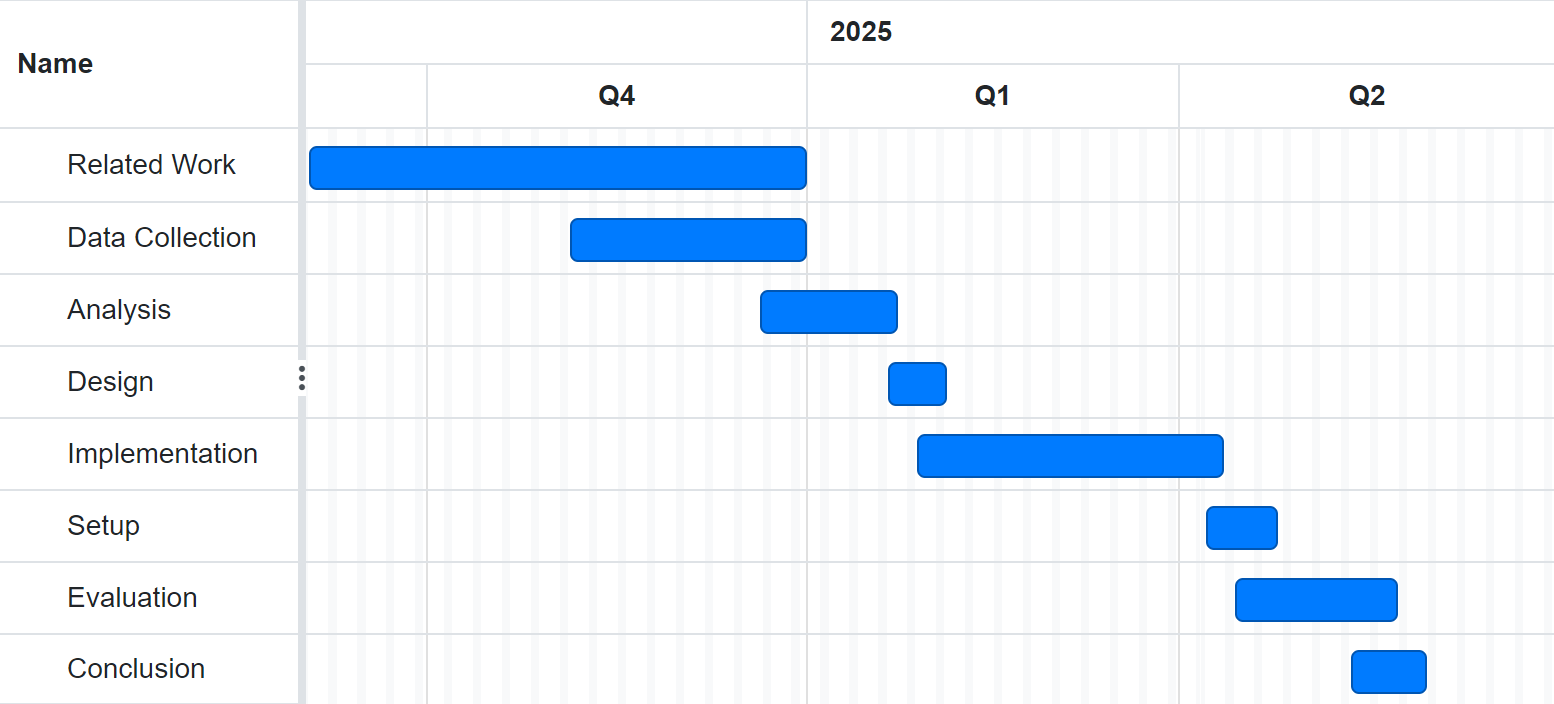
\includegraphics[width=1.8\columnwidth]{Gantt}
				}
			}
		\end{center}
		\caption{Gantt Diagram over the expected task for the project}
		\label{img:Gantt}
	\end{figure}
\end{document}